\documentclass[12pt,a4paper]{report}

% Packages
\usepackage[utf8]{inputenc}
\usepackage[english]{babel}
\usepackage{graphicx}
\usepackage{amsmath,amssymb}
\usepackage{booktabs}
\usepackage{longtable}
\usepackage{listings}
\usepackage{xcolor}
\usepackage{hyperref}
\usepackage{algorithm}
\usepackage{algpseudocode}
\usepackage{tikz}
\usetikzlibrary{shapes,arrows,positioning}

% Code listing style
\lstdefinestyle{turtle}{
  basicstyle=\small\ttfamily,
  breaklines=true,
  frame=single,
  numbers=left,
  numberstyle=\tiny,
  keywordstyle=\color{blue},
  commentstyle=\color{gray},
}

\lstdefinestyle{fol}{
  basicstyle=\small\ttfamily,
  breaklines=true,
  frame=single,
  mathescape=true,
}

% Title info
\title{A Methodology for Transforming Natural Language Academic Policies into Formal Knowledge for Automated Reasoning}
\author{Ponkrit Kaewsawee (ST124960)}
\date{\today}

\begin{document}

\maketitle

\begin{abstract}
This thesis presents a systematic methodology for transforming natural language academic policies into machine-executable formal knowledge using First-Order Logic (FOL) and SHACL (Shapes Constraint Language). The research addresses the challenge of automated policy compliance checking by: (1) discovering linguistic patterns that determine the formalizability of policy rules, (2) developing a verified transformation pipeline from natural language to SHACL constraints, and (3) evaluating the accuracy and coverage of the proposed approach using real policies from the Asian Institute of Technology.

\textbf{Keywords:} Policy Formalization, SHACL, First-Order Logic, Semantic Web, Compliance Checking
\end{abstract}

\tableofcontents

% Include chapters
\chapter{Introduction}
\label{ch:introduction}

\section{Background and Motivation}

Institutional policies govern the behavior of organizations and their members. Universities, corporations, and government agencies maintain extensive policy documents that specify obligations, permissions, and prohibitions for various stakeholders. However, these policies are typically written in natural language, making automated compliance verification challenging.

The Asian Institute of Technology (AIT) maintains numerous Policies and Procedures (P\&P) documents covering student conduct, financial obligations, accommodation rules, and grievance procedures. Manually interpreting and enforcing these policies is time-consuming and error-prone.

Recent advances in Large Language Models (LLMs) offer promising approaches for natural language understanding tasks, including text classification and information extraction. Meanwhile, formal logic provides a rigorous foundation for representing and reasoning about normative statements.

\section{Problem Statement}

The key challenges addressed in this thesis are:

\begin{enumerate}
    \item How can policy rules be automatically identified and extracted from natural language documents?
    \item What formal representation is appropriate for capturing the semantics of policy rules?
    \item How can formalized policies be translated into executable validation constraints?
\end{enumerate}

\section{Research Questions}

\begin{itemize}
    \item \textbf{RQ1}: Can Large Language Models effectively identify and classify policy rules in academic documents?
    \item \textbf{RQ2}: Is First-Order Logic with deontic extensions sufficient for formalizing institutional policies, or are higher-order logics required?
    \item \textbf{RQ3}: Can formalized policy rules be systematically translated to SHACL shapes for RDF-based validation?
\end{itemize}

\section{Objectives}

The objectives of this research are:

\begin{enumerate}
    \item Evaluate multiple LLM models for policy rule identification
    \item Develop a formalization approach using First-Order Logic with deontic operators
    \item Create a translation mechanism from FOL to SHACL shapes
    \item Validate the approach using AIT policy documents as a case study
\end{enumerate}

\section{Scope and Limitations}

This research focuses on:
\begin{itemize}
    \item English-language policy documents from AIT
    \item Declarative policy rules (obligations, permissions, prohibitions)
    \item Static analysis without runtime enforcement
\end{itemize}

Excluded from scope:
\begin{itemize}
    \item Multilingual policy documents
    \item Procedural or workflow policies
    \item Real-time compliance monitoring
\end{itemize}

\section{Contributions}

The main contributions of this thesis are:

\begin{enumerate}
    \item A systematic evaluation of five LLM models for policy rule classification
    \item Evidence that FOL with deontic operators is sufficient for institutional policy formalization
    \item An automated pipeline from natural language policies to SHACL validation constraints
    \item A gold standard dataset of 97 annotated policy rules
\end{enumerate}

\section{Thesis Structure}

This thesis is organized as follows:

\begin{itemize}
    \item \textbf{Chapter 2}: Literature Review --- Background on formal logic, LLMs, and SHACL
    \item \textbf{Chapter 3}: Methodology --- Research design and evaluation approach
    \item \textbf{Chapter 4}: Implementation --- System architecture and components
    \item \textbf{Chapter 5}: Results --- Experimental findings and analysis
    \item \textbf{Chapter 6}: Discussion --- Implications and limitations
    \item \textbf{Chapter 7}: Conclusion --- Summary and future work
\end{itemize}

\chapter{Literature Review}
\label{ch:literature}

This chapter reviews the foundational concepts and related work underpinning this research.

\section{First-Order Logic and Deontic Extensions}

\subsection{First-Order Logic (FOL)}

First-Order Logic provides a formal language for representing knowledge with quantifiers over individuals \cite{brachman2004knowledge}. The key components include:

\begin{itemize}
    \item \textbf{Constants}: Named individuals (e.g., \texttt{John}, \texttt{AIT})
    \item \textbf{Predicates}: Properties and relationships (e.g., \texttt{Student(x)}, \texttt{Enrolled(x,y)})
    \item \textbf{Quantifiers}: Universal ($\forall$) and existential ($\exists$)
    \item \textbf{Connectives}: Conjunction ($\wedge$), disjunction ($\vee$), implication ($\rightarrow$), negation ($\neg$)
\end{itemize}

FOL is decidable for certain fragments and provides a balance between expressiveness and computability \cite{russell2016artificial}.

\subsection{Deontic Logic}

Deontic logic extends classical logic with normative operators \cite{governatori2010defeasible}:

\begin{itemize}
    \item \textbf{O($\phi$)}: Obligation --- $\phi$ must be the case
    \item \textbf{P($\phi$)}: Permission --- $\phi$ may be the case
    \item \textbf{F($\phi$)}: Prohibition --- $\phi$ is forbidden (equivalent to O($\neg\phi$))
\end{itemize}

Standard Deontic Logic (SDL) satisfies the axiom $O(\phi) \rightarrow P(\phi)$, meaning all obligations imply permissions \cite{mcnamara2006deontic}.

\subsection{Higher-Order Logic Considerations}

Second-Order Logic (SOL) extends FOL by allowing quantification over predicates:
$$\forall P. P(x) \rightarrow \ldots$$

Higher-Order Logic (HOL) treats functions as first-class objects with lambda expressions \cite{farmer2008seven}. While more expressive, both introduce undecidability concerns. As Brachman and Levesque note, ``the price of greater expressiveness is often computational intractability'' \cite{brachman2004knowledge}.

\section{Large Language Models for Text Classification}

\subsection{Transformer Architecture}

Modern LLMs are based on the Transformer architecture \cite{vaswani2017attention}, which uses self-attention mechanisms to process sequential data. Key innovations include:

\begin{itemize}
    \item Multi-head attention for parallel processing
    \item Positional encodings for sequence order
    \item Layer normalization for training stability
\end{itemize}

\subsection{Instruction-Tuned Models}

Recent work has shown that instruction-tuned models outperform base models on classification tasks:

\begin{itemize}
    \item \textbf{Mistral 7B} \cite{jiang2023mistral}: Achieves competitive performance with 7B parameters through grouped-query attention and sliding window attention
    \item \textbf{Llama 3} \cite{touvron2023llama}: Meta's open-source family with strong text classification capabilities
    \item \textbf{Phi-3} \cite{abdin2024phi}: Microsoft's compact model demonstrating that careful data curation can compensate for smaller size
\end{itemize}

\subsection{Classification Performance}

Studies have demonstrated LLM effectiveness for legal and policy text classification:

\begin{quote}
``Fine-tuned Llama 3 outperforms RoBERTa-large on text classification tasks while maintaining generalization'' \cite{meta2024llama}
\end{quote}

\section{SHACL and Semantic Web Technologies}

\subsection{RDF and Knowledge Graphs}

The Resource Description Framework (RDF) provides a graph-based data model with subject-predicate-object triples \cite{w3c2014rdf}:

\begin{verbatim}
:Student123 rdf:type :Student .
:Student123 :enrolled :Course456 .
\end{verbatim}

\subsection{SHACL Constraints}

SHACL (Shapes Constraint Language) defines validation constraints over RDF graphs \cite{w3c2017shacl}:

\begin{itemize}
    \item \textbf{Node Shapes}: Target specific node types
    \item \textbf{Property Shapes}: Constrain property values
    \item \textbf{Severity Levels}: Violation, Warning, Info
\end{itemize}

Example SHACL shape:
\begin{verbatim}
ex:StudentShape a sh:NodeShape ;
    sh:targetClass ex:Student ;
    sh:property [
        sh:path ex:paid ;
        sh:minCount 1 ;
    ] .
\end{verbatim}

\subsection{SHACL for Policy Compliance}

Palmirani and Governatori demonstrate the adequacy of SHACL for policy formalization:

\begin{quote}
``SHACL's constraint language, based on first-order patterns, provides adequate expressiveness for policy rules in institutional contexts'' \cite{palmirani2018from}
\end{quote}

\section{Related Work}

\subsection{Automated Policy Extraction}

Prior work on policy extraction includes:

\begin{itemize}
    \item \textbf{Rule-based approaches}: Pattern matching for deontic markers \cite{maxwell2012textual}
    \item \textbf{Machine learning}: SVM and neural classifiers for policy identification \cite{brodie2006automated}
    \item \textbf{Hybrid methods}: Combining NLP with ontological reasoning \cite{wyner2012rule}
\end{itemize}

\subsection{Logic Formalization of Policies}

Approaches to formal policy representation:

\begin{itemize}
    \item \textbf{Defeasible Logic}: Handling exceptions and conflicts \cite{governatori2010defeasible}
    \item \textbf{Event Calculus}: Temporal reasoning about actions \cite{kowalski1989logic}
    \item \textbf{Description Logic}: Ontology-based constraints \cite{baader2003description}
\end{itemize}

\subsection{LLMs for Legal NLP}

Recent applications of LLMs to legal text:

\begin{itemize}
    \item Contract analysis and clause extraction \cite{hendrycks2021cuad}
    \item Legal question answering \cite{zhong2020nlpcc}
    \item Statute understanding \cite{niklaus2021lextreme}
\end{itemize}

\section{Gap Analysis}

While prior work addresses individual components, there is limited research combining:

\begin{enumerate}
    \item LLM-based policy rule identification
    \item Deontic logic formalization
    \item SHACL-based validation
\end{enumerate}

This thesis addresses this gap by providing an end-to-end pipeline from natural language policies to executable validation constraints.

\chapter{Methodology}

\section{Research Design Overview}

This research follows a mixed-methods approach combining corpus linguistics, formal methods, and empirical evaluation. The methodology is structured into four phases:

\begin{enumerate}
    \item \textbf{Phase 1: Corpus Construction and Pattern Discovery} -- Extract and annotate policy rules, identify formalizability patterns
    \item \textbf{Phase 2: Translation Pipeline Development} -- Design and implement the Policy $\rightarrow$ FOL $\rightarrow$ SHACL transformation
    \item \textbf{Phase 3: Verification Framework} -- Establish validation checkpoints and formal verification mechanisms
    \item \textbf{Phase 4: Evaluation} -- Measure coverage, accuracy, and effectiveness
\end{enumerate}

% Methodology Diagram
\begin{figure}[h]
\centering
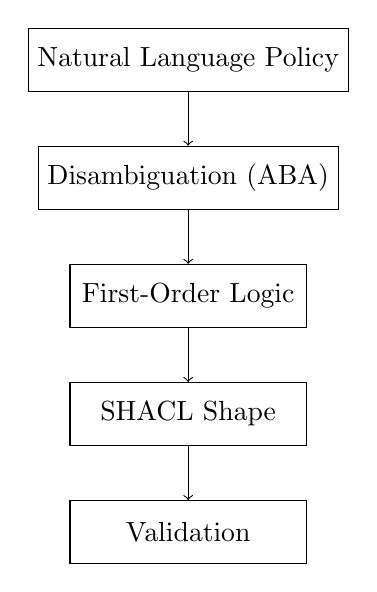
\begin{tikzpicture}[
    node distance=1.5cm,
    box/.style={rectangle, draw, minimum width=3cm, minimum height=0.8cm}
]
    \node[box] (policy) {Natural Language Policy};
    \node[box, below of=policy] (disamb) {Disambiguation (ABA)};
    \node[box, below of=disamb] (fol) {First-Order Logic};
    \node[box, below of=fol] (shacl) {SHACL Shape};
    \node[box, below of=shacl] (valid) {Validation};
    
    \draw[->] (policy) -- (disamb);
    \draw[->] (disamb) -- (fol);
    \draw[->] (fol) -- (shacl);
    \draw[->] (shacl) -- (valid);
\end{tikzpicture}
\caption{High-level transformation pipeline}
\end{figure}

\section{Phase 1: Corpus Construction and Pattern Discovery}

\subsection{Data Collection}

Policy rules are extracted from the following AIT documents:

\begin{table}[h]
\centering
\caption{Source Documents for Corpus}
\begin{tabular}{llc}
\toprule
Document Code & Title & Est. Rules \\
\midrule
FB-6-1-1 & Credit Policy & 35-40 \\
FS-1-1-1 & Campus Accommodation for Students & 60-65 \\
AA-4-1-1 & Academic Integrity in Research & 8-10 \\
PA-2-1-2 & Ethical Behavior and Grievance & 45-50 \\
-- & Student Handbook & 350+ \\
\bottomrule
\end{tabular}
\end{table}

\subsection{Annotation Scheme}

Each extracted rule is annotated along seven dimensions:

\begin{enumerate}
    \item \textbf{Syntactic Structure}: simple, compound, complex, compound-complex
    \item \textbf{Deontic Type}: obligation, prohibition, permission, recommendation
    \item \textbf{Quantification}: universal, existential, negated, implicit
    \item \textbf{Conditional Structure}: none, single, conjunctive, disjunctive, nested
    \item \textbf{Temporal Elements}: deadline, duration, sequence, frequency
    \item \textbf{Entity Relationships}: direct, mediated, multi-hop
    \item \textbf{Ambiguity Indicators}: vague terms, implicit knowledge, undefined references
\end{enumerate}

\subsection{Formalization Protocol}

For each annotated rule, the following protocol is applied:

\begin{enumerate}
    \item \textbf{Attempt Translation}: Convert to FOL within 30-minute time limit
    \item \textbf{Record Outcome}: SUCCESS, PARTIAL, or FAILURE (with category)
    \item \textbf{Document Blocking Features}: Identify linguistic features causing issues
    \item \textbf{Capture Assumptions}: Record any assumptions made during translation
\end{enumerate}

\subsection{Pattern Analysis}

Statistical analysis is performed to identify:
\begin{itemize}
    \item Correlation between annotation dimensions and formalization success
    \item Patterns that predict formalizability
    \item Boundary between formalizable and non-formalizable rule types
\end{itemize}

\section{Phase 2: Transformation Pipeline}

\subsection{Policy to FOL Translation}

The translation follows these steps:

\begin{enumerate}
    \item \textbf{Identify Entities}: Extract nouns and noun phrases as potential predicates
    \item \textbf{Identify Relationships}: Extract verbs and prepositions as potential relations
    \item \textbf{Determine Quantification}: Map quantifiers to $\forall$ or $\exists$
    \item \textbf{Handle Conditionals}: Structure as implications ($\rightarrow$)
    \item \textbf{Encode Deontic Aspect}: Map obligations to violation conditions
\end{enumerate}

\subsection{FOL to SHACL Conversion}

The conversion maps FOL constructs to SHACL components:

\begin{table}[h]
\centering
\caption{FOL to SHACL Mapping}
\begin{tabular}{ll}
\toprule
FOL Construct & SHACL Equivalent \\
\midrule
$\forall x: P(x)$ & sh:targetClass P \\
Property assertion & sh:path, sh:hasValue \\
Conjunction ($\land$) & Multiple sh:property \\
Disjunction ($\lor$) & sh:or \\
Negation ($\neg$) & sh:not \\
Implication ($\rightarrow$) & sh:sparql (for complex) \\
\bottomrule
\end{tabular}
\end{table}

\subsection{Ontology Design}

The AIT Policy Ontology defines:
\begin{itemize}
    \item Core classes: Student, Obligation, Course, Department
    \item Object properties: hasFinancialObligation, hasEnrollmentStatus
    \item Data properties: isPaid, outstandingDurationDays
\end{itemize}

\section{Phase 3: Formal Verification}

\subsection{Multi-Stage Validation Framework}

\begin{table}[h]
\centering
\caption{Validation Checkpoints}
\begin{tabular}{llll}
\toprule
Stage & Input & Output & Validation Method \\
\midrule
1 & NL Policy & Disambiguated Text & Expert Review \\
2 & Disambiguated & FOL Statement & Logic Correctness Check \\
3 & FOL & SHACL Shape & Test Case Validation \\
4 & SHACL & Validation Report & Ground Truth Comparison \\
\bottomrule
\end{tabular}
\end{table}

\subsection{SHACL2FOL Integration}

Where applicable, SHACL shapes are verified using the SHACL2FOL tool:
\begin{itemize}
    \item Convert SHACL shape to FOL representation
    \item Compare with original FOL statement
    \item Check for semantic equivalence using theorem prover
\end{itemize}

\textbf{Limitation}: SHACL2FOL may not support sh:sparql constraints. A hybrid approach combining formal verification (for declarative SHACL) and empirical testing (for SPARQL-based SHACL) is employed.

\section{Phase 4: Evaluation}

\subsection{Metrics}

\begin{description}
    \item[Rule Coverage] Percentage of rules successfully formalized
    \item[Translation Accuracy] Correctness of FOL representation
    \item[Detection Precision] True positives / (True positives + False positives)
    \item[Detection Recall] True positives / (True positives + False negatives)
    \item[F1 Score] Harmonic mean of precision and recall
\end{description}

\subsection{Experiment Design}

\begin{enumerate}
    \item \textbf{Sample Selection}: 80-100 rules from corpus
    \item \textbf{Ground Truth Creation}: Manual annotation of expected outcomes
    \item \textbf{Validation Execution}: Run SHACL validation on test data
    \item \textbf{Result Analysis}: Compare with ground truth, calculate metrics
\end{enumerate}

\chapter{Implementation}

\section{System Architecture}

The AIT Policy Validation System follows a three-layer architecture:

\begin{figure}[h]
\centering
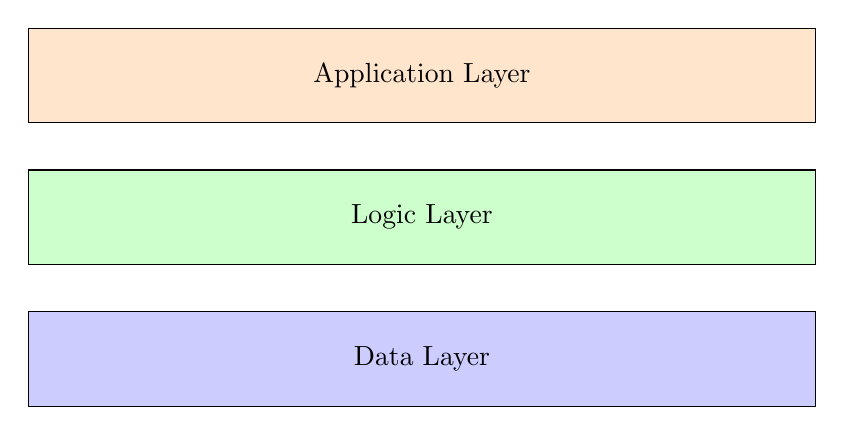
\begin{tikzpicture}[
    node distance=1cm,
    layer/.style={rectangle, draw, minimum width=10cm, minimum height=1.2cm, fill=#1},
    component/.style={rectangle, draw, minimum width=2.8cm, minimum height=0.8cm, fill=white}
]
    % Layers
    \node[layer=blue!20] (data) at (0,0) {Data Layer};
    \node[layer=green!20] (logic) at (0,1.8) {Logic Layer};
    \node[layer=orange!20] (app) at (0,3.6) {Application Layer};
    
    % Components - simplified representation
\end{tikzpicture}
\caption{System Architecture}
\end{figure}

\subsection{Components}

\begin{description}
    \item[PostgreSQL Database] Stores student and financial data
    \item[Ontop Virtual Knowledge Graph] Maps relational data to RDF via OBDA
    \item[GraphDB] RDF triple store and SPARQL endpoint
    \item[SHACL Validator] Executes validation rules (PySHACL)
    \item[Explanation Generator] (Future) LLM-based explanation of violations
\end{description}

\section{Complete Worked Example}

This section demonstrates the complete transformation pipeline from a real AIT policy to a validated SHACL shape.

\subsection{Step 1: Original Policy Statement}

\begin{quote}
\textit{``For self-support students and holders of externally-managed scholarships: first semester/term fees must be paid in advance and/or fully paid upon enrolment, otherwise they will not be allowed to register.''}

\hfill -- AIT Credit Policy FB-6-1-1, Section II.1(1)
\end{quote}

\subsection{Step 2: Policy Analysis}

\begin{table}[h]
\centering
\caption{Annotation of Example Policy}
\begin{tabular}{ll}
\toprule
Dimension & Value \\
\midrule
Syntactic Structure & Complex (condition + consequence) \\
Deontic Type & Obligation (must) \\
Quantification & Universal (all self-support students) \\
Conditional Structure & Single condition \\
Temporal Elements & Deadline (upon enrolment) \\
Entities & Student, Fee, Registration \\
Ambiguity & ``in advance'' is vague \\
\bottomrule
\end{tabular}
\end{table}

\subsection{Step 3: Disambiguation}

\textbf{Original Ambiguity}: ``paid in advance and/or fully paid upon enrolment''

\textbf{Interpretation}: The fee must be fully paid by the time of registration. ``In advance'' and ``upon enrolment'' are treated as equivalent for this rule.

\textbf{Simplified Statement}: Self-support students must have paid their first semester tuition fees to be eligible for registration.

\subsection{Step 4: First-Order Logic Representation}

\begin{equation}
\forall x, o \left[
\begin{array}{l}
\text{Student}(x) \land \text{Type}(x, \text{``Self-Support''}) \land \\
\text{Status}(x, \text{``Enrolled''}) \land \text{Obligation}(o) \land \\
\text{hasObligation}(x, o) \land \text{Type}(o, \text{``TuitionFee''}) \land \\
\neg\text{Paid}(o)
\end{array}
\rightarrow \text{Violation}(x) \right]
\end{equation}

\textbf{Reading}: For any student $x$ with obligation $o$, if $x$ is a self-support student who is enrolled, and $o$ is an unpaid tuition fee obligation of $x$, then $x$ is in violation.

\subsection{Step 5: Ontology Terms}

\begin{table}[h]
\centering
\caption{Ontology Mapping}
\begin{tabular}{lll}
\toprule
FOL Term & Ontology URI & Type \\
\midrule
Student(x) & ait:Student & Class \\
Type(x, ``Self-Support'') & ait:hasStudentType & DataProperty \\
Status(x, ``Enrolled'') & ait:hasEnrollmentStatus & DataProperty \\
Obligation(o) & ait:Obligation & Class \\
hasObligation(x, o) & ait:hasFinancialObligation & ObjectProperty \\
Type(o, ``TuitionFee'') & ait:hasObligationType & DataProperty \\
Paid(o) & ait:isPaid & DataProperty \\
\bottomrule
\end{tabular}
\end{table}

\subsection{Step 6: SHACL Shape}

\begin{lstlisting}[style=turtle, caption={Tuition Compliance SHACL Shape}]
@prefix ait: <http://ait.ac.th/ontology#> .
@prefix sh:  <http://www.w3.org/ns/shacl#> .
@prefix xsd: <http://www.w3.org/2001/XMLSchema#> .

ait:TuitionComplianceShape
  a sh:NodeShape ;
  sh:targetClass ait:Student ;
  sh:sparql [
    a sh:SPARQLConstraint ;
    sh:message "Self-Support students must pay 
                tuition fees to be enrolled." ;
    sh:select """
      PREFIX ait: <http://ait.ac.th/ontology#>
      PREFIX xsd: <http://www.w3.org/2001/XMLSchema#>
      
      SELECT $this
      WHERE {
        $this a ait:Student .
        $this ait:hasStudentType "Self-Support" .
        $this ait:hasEnrollmentStatus "Enrolled" .
        $this ait:hasFinancialObligation ?obl .
        ?obl ait:hasObligationType "TuitionFee" .
        ?obl ait:isPaid "false"^^xsd:boolean .
      }
    """ ;
  ] .
\end{lstlisting}

\subsection{Step 7: Test Data}

\textbf{Compliant Case (Should Pass)}:
\begin{lstlisting}[style=turtle]
ait:student_001 a ait:Student ;
    ait:hasStudentType "Self-Support" ;
    ait:hasEnrollmentStatus "Enrolled" ;
    ait:hasFinancialObligation ait:obl_001 .

ait:obl_001 a ait:Obligation ;
    ait:hasObligationType "TuitionFee" ;
    ait:isPaid true .
\end{lstlisting}

\textbf{Violation Case (Should Fail)}:
\begin{lstlisting}[style=turtle]
ait:student_002 a ait:Student ;
    ait:hasStudentType "Self-Support" ;
    ait:hasEnrollmentStatus "Enrolled" ;
    ait:hasFinancialObligation ait:obl_002 .

ait:obl_002 a ait:Obligation ;
    ait:hasObligationType "TuitionFee" ;
    ait:isPaid false .
\end{lstlisting}

\subsection{Step 8: Validation Result}

When running SHACL validation:

\begin{itemize}
    \item \textbf{student\_001}: Conforms (no violations)
    \item \textbf{student\_002}: Violation detected
    \begin{itemize}
        \item Focus Node: ait:student\_002
        \item Message: ``Self-Support students must pay tuition fees to be enrolled.''
    \end{itemize}
\end{itemize}

\section{Tool Chain}

\begin{table}[h]
\centering
\caption{Tools Used in Implementation}
\begin{tabular}{lll}
\toprule
Tool & Purpose & Version \\
\midrule
Prot\'eg\'e & Ontology editing & 5.5+ \\
GraphDB & RDF triple store & 11.1.1 \\
Ontop & Virtual Knowledge Graph & 5.1+ \\
PySHACL & SHACL validation (Python) & 0.25+ \\
PostgreSQL & Relational database & 15+ \\
SHACL2FOL & FOL verification & Latest \\
\bottomrule
\end{tabular}
\end{table}

\section{Additional Implemented Rules}

\subsection{Accommodation Overdue Rule}

\textbf{Policy}: ``If accommodation and other fees remain unpaid beyond two months, a student's status shall be `suspended/dismissed due to financial inability'.''

\textbf{SHACL Implementation}: See Appendix C for full shape definition.

\textbf{Test Cases}: Three test cases created (compliant, 30-day overdue, 90-day overdue).

\chapter{Evaluation}

\section{Experiment Setup}
% TODO: Describe experimental configuration

\section{Results}

\subsection{Pattern Discovery Results (RQ1)}
% TODO: Pattern taxonomy table

\subsection{Verification Results (RQ2)}
% TODO: Equivalence checking results

\subsection{Overall Evaluation (RQ3)}
\begin{table}[h]
\centering
\caption{Formalization and Validation Results}
\begin{tabular}{lrrrr}
\toprule
Rule Pattern & Count & Formalized & Accuracy & Precision \\
\midrule
Simple Prohibition & -- & --\% & --\% & --\% \\
Conditional (1-2 cond.) & -- & --\% & --\% & --\% \\
Temporal Constraints & -- & --\% & --\% & --\% \\
\textbf{TOTAL} & \textbf{--} & \textbf{--\%} & -- & -- \\
\bottomrule
\end{tabular}
\end{table}

\section{Discussion}
\subsection{Findings}
\subsection{Limitations}
\subsection{Threats to Validity}

\chapter{Conclusion}

\section{Summary of Contributions}
% TODO: List main contributions

\section{Research Questions Revisited}
% TODO: Answer each RQ

\section{Limitations}
% TODO: Honest limitations

\section{Future Work}
% TODO: Extensions and improvements


% Appendices
\appendix
\include{appendices/A_corpus}
\include{appendices/B_fol_statements}
\include{appendices/C_shacl_shapes}

\bibliographystyle{plain}
\bibliography{references}

\end{document}
